
Gli effetti principali delle radiazioni su dispositivi elettronici possono essere di due categorie \cite{bib:Effetti_Radiazioni_1987}:
\begin{itemize}
	\item Danno da spostamento {(\textit{DD})}, ovvero la dislocazione degli atomi dai loro siti reticolari,
	\item Ionizzazione, ovvero la generazione di coppie elettrone-lacuna ($e-h$).
\end{itemize}

\subsection{Danno da spostamento}
Quando una particella (tipicamente un neutrone, ma non solo) possiede abbastanza energia da poter dislocare un atomo al di fuori dalla sua posizione normale all'interno reticolo, avviene il danno da spostamento (\textit{Displacement Damage}); ne risulta che le caratteristiche elettroniche del materiale vengano alterate.
Inoltre, può verificarsi che l'atomo colpito generi a sua volta altri \textit{DD}, a patto che abbia abbastanza energia. L'energia minima da trasferire a un atomo affinché si generi un danno da spostamento nel silicio è di $20 eV$.
% Preso da Slide di Valerio Re

% Il danno da spostamento dipende dall'energia della particella, in particolare i protoni, avendo una massa maggiore, consentono di trasferire all'atomo colpito una energia maggiore \cite{bib:Effetti_Radiazioni_su_dispositivi_optoeltronici}.

\vspace*{0.5cm}

Siccome nei MOSFET la conduzione delle cariche avviene a livello superficiale e non nel substrato, il danno da spostamento non è molto rilevante. La ionizzazione, invece, può comportare variazioni dei parametri elettrici come guadagno e tensione di soglia; per questo motivo in questo lavoro ci concentreremo solo sugli effetti della ionizzazione.

% \vspace{0.5cm}
 
% Il passaggio di una particella ionizzante all'interno della materia, comporta una perdita di energia.
% Questa dissipazione può essere formalizzata come \todo[inlinepar]{Presa da: "Radiation\_Effects\_and\_RHA\_ESA\_Course\_9-10\_May\_2017\_TID\_MP\_FINAL\_WIN.pdf" slide 5}:
% $$ \Delta E = \Delta E_{\text{elettronica}} + \Delta E_{nucleare} $$
% La \textbf{perdita di energia elettronica} è dovuta dalle interazioni con gli elettroni negli atomi, mentre la \textbf{perdita di energia nucleare} è causata dalle interazioni con i nuclei degli atomi.
% Gran parte dell'energia persa è elettronica, poiché solo occasionalmente avvengono \textit{collisioni forti} tali da creare frammenti nucleari. Pertanto la perdita di energia totale è una buona approssimazione della perdita dell'energia elettronica \cite{bib:Effetti_Radiazioni_NASA}.

\vspace{0.5cm}

\subsection{Ionizzazione}\label{cap1:ionizzazione}
La creazione di coppie $e-h$ (\textit{electron-hole}) all'interno del dispositivo MOSFET è provocata dalla ionizzazione, che a sua volta è generata dal passaggio di una o più particelle che depositano una certa quantità di energia nel materiale. Esiste una proporzionalità diretta tra il numero di coppie elettrone-lacuna e l'energia depositata da parte della particella che collide con il dispositivo. Per esempio, nel silicio si ha una constante di $\frac{1}{3,6eV}$ mentre per il biossido di silicio è di $\frac{1}{18eV}$ \cite{bib:Effetti_Radiazioni_NASA}.


% Il passaggio di una particella all'interno della struttura del MOSFET, rilascia una certa quantità di energia provocando la ionizzazione


% Esiste una proporzionalità diretta tra il numero di coppie $e-h$ e l'\textbf{energia elettronica persa} da parte della particella che collide con il dispositivo. Per esempio, nel silicio si ha una constante di $\frac{1}{3,6eV}$ mentre per il biossido di silicio è di $\frac{1}{18eV}$ \cite{bib:Effetti_Radiazioni_NASA}.

\vspace{0.5cm}

Negli isolanti, come l'ossido di \emph{gate} dei transistori MOSFET, l'effetto della ionizzazione è cumulativo. Gli elettroni liberati da una particella ionizzante si possono muovere facilmente, soprattutto grazie a effetti di campo dovuti, ad esempio, a polarizzazioni.
Al contrario, le lacune sono molto meno mobili, dai 5 ai 12 ordini di grandezza inferiori rispetto agli elettroni. La maggior parte delle lacune riesce a sopravvivere alla ricombinazione con gli elettroni, creando perciò una carica positiva vicino alla giunzione $Si/SiO_2$.
La carica intrappolata nell'ossido ha come effetto un aumento (in valore assoluto) della tensione di soglia dei MOSFET a canale P; mentre negli NMOS l'effetto è un po' più complesso e dipende dai seguenti fattori:
\begin{enumerate}
	\item Cariche positive intrappolate nell'ossido
	\item Cariche negative presenti nelle trappole all'interfaccia\footnote{Le trappole all'interfaccia sono dovute a imperfezioni o difetti presenti alla giunzione $Si/SiO_2$ che possono intrappolare delle cariche. Queste trappole aumentano all'aumentare della dose assorbita.}
\end{enumerate}
Mentre la prima comporta una riduzione della tensione di soglia, la seconda ne provoca un aumento, in quanto la carica intrappolata all'interfaccia è negativa (negli NMOS si ha moto di elettroni nel canale). 
È inoltre opportuno sottolineare che anche nei PMOS vi sono portatori intrappolati all'interfaccia $Si/SiO_2$. Ma questi portatori, al contrario di quanto accade per gli NMOS, hanno carica positiva e pertanto le cariche intrappolate hanno un effetto che si somma a quello dovuto alle cariche positive intrappolate nell'ossido di \textit{gate}.  

\vspace{0.5cm}

Un altro effetto presente solo negli NMOS è quello della formazione di transistor parassiti \cite{effetti_radiazioni:CMOS_IC_radiation_hardening_by_design}. Questo effetto è dovuto all'accumulo delle cariche positive nella \textit{Shallow Trench Isolation} (\textit{STI}), il quale crea un canale conduttivo tra \emph{source} e \emph{drain} che aggira quello principale (figura \ref{fig:accumulo_lacune_STI}). Questo collegamento fa sì che possa esserci un flusso di corrente anche quando il dispositivo è polarizzato con una $V_{GS} \simeq 0$.

\begin{figure}[ht]
	\centering

	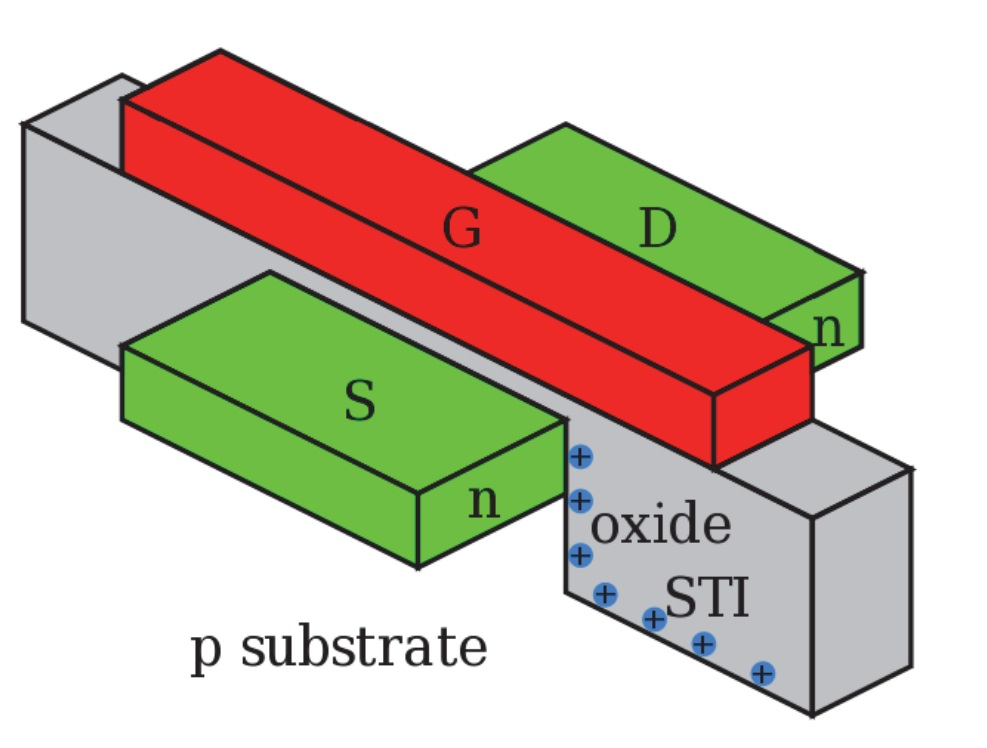
\includegraphics[width = 0.5 \textwidth]{capitolo1/effettiRadiazioniIonizzanti/Holes-trapped-in-the-shallow-trench-isolation-STI.jpg}

	\caption[Lacune nella \textit{STI}]{Accumulo delle lacune nella \textit{shallow trench isolation} \cite{effetti_radiazioni:CMOS_IC_radiation_hardening_by_design}.}
	\label{fig:accumulo_lacune_STI}

\end{figure}

\vspace*{0.5cm}

Poiché gli effetti delle radiazioni sui MOSFET precedentemente elencati sono maggiori sui dispositivi a canale N, in passato si è consolidata la preferenza a utilizzare i PMOS come transistori d'ingresso in preamplificatori di carica a basso rumore, essendo più tolleranti alla ionizzazione. L'evoluzione di tecnologie MOSFET, che ha portato alla fabbricazione di transistori con dimensioni minime di canale sempre più piccole (figura \ref{fig:scaling_mosfet}), ha comportato, grazie alla riduzione dello spessore dell'ossido di \textit{gate}, un aumento della resistenza alle radiazioni ionizzanti.  

\begin{figure}[ht]
	\centering

	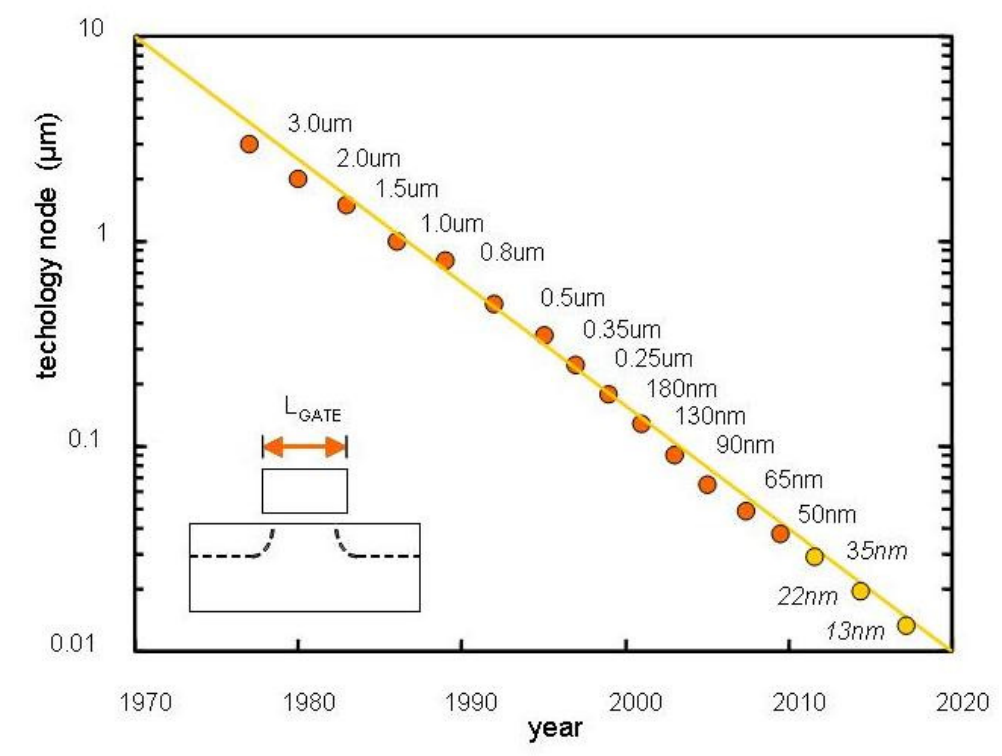
\includegraphics[width = 0.60\linewidth]{capitolo1/effettiRadiazioniIonizzanti/scaling_mosfet.png}
	\caption[Scaling dei dispositivi elettronici]{Evoluzione delle dimensioni nei dispositivi elettronici \cite{effetti_radiazioni_scaling:Nanoelectronics_and_nanolithography}}
	\label{fig:scaling_mosfet}
\end{figure}


\vspace{0.5cm}

Gli effetti del danno da ionizzazione si riducono con il tempo (settimane, mesi, anni) e questo effetto è denominato \emph{annealing}. Per simulare il ripristino delle prestazioni elettroniche dei dispositivi in un tempo ragionevolmente breve, si effettua un \emph{annealing} ad alta temperatura, tipicamente $100\degree C$ per 24 ore, per accelerarne i meccanismi.

\subsection{Misura della dose}
La quantità di radiazioni ionizzanti assorbite da un materiale viene chiamata \textit{TID} (\textit{Total Ionizing Dose}) ed è espressa in energia su unità di massa.
La \textit{TID} normalmente è misurata in $rad$ (\textit{radiation absorbed dose}), definito come $100 erg  = 100 \cdot 10^{-7} J$ per grammo di materiale. Un'altra unità di misura per la \textit{TID}, accolta anche dal Sistema Internazionale, sono i \textit{gray} ($Gy$), dove $1 Gy = 100rad = 1\frac{J}{Kg}$.
Data l'esistenza di una dipendenza tra la quantità di energia persa e il materiale su cui essa si deposita, spesso insieme all'unità di misura si indica anche il materiale; ad esempio, nel caso del biossido di silicio si indica $rad(SiO_{2})$. 




